\section{Quantum Circuits}

\textbf{4.1}

The normalized eigenvectors of $X$ is $ \left(\frac{1}{\sqrt{2}}(1,1),\frac{1}{\sqrt{2}}(1,-1)\right)$. The eigenvector $\frac{1}{\sqrt{2}}(1,1)$ can be expressed as
\[\ket{D}=\frac{1}{\sqrt{2}}\ket{0} + \frac{1}{\sqrt{2}}\ket{1}\]
This means $ \cos(\theta/2) = \frac{1}{\sqrt{2}}$ and $e^{i\varphi}\sin(\theta/2) = \frac{1}{\sqrt{2}}$ and so $\theta/2 = \pi/4$ resulting in $ \theta = \pi/2$. That makes $\sin(\theta/2) =\frac{1}{\sqrt{2}}$ and so $e^{i\varphi}\sin(\theta/2)  = e^{i\varphi}\frac{1}{\sqrt{2}}$ resulting in $\varphi = 0$. This means we have the Bloch vector of $ (1,0,0)$ for $\ket{D}$. The eigenvector $\frac{1}{\sqrt{2}}(1,-1)$ can be expressed as 
\[\ket{E} = \frac{1}{\sqrt{2}}\ket{0} - \frac{1}{\sqrt{2}}\ket{1}\]
In this case we would have $\theta = \pi/2$ but we must have $ e^{i\varphi} = -1$ and so $\varphi = \pi$. Thus we have $(-1,0,0)$ as the Bloch vector for $\ket{E}$

The normalized eigenvectors of $Y$ is $ \left(\frac{1}{\sqrt{2}}(1,-i),\frac{1}{\sqrt{2}}(1,i)\right)$. We can express the first eigenvector as
\[\ket{F} = \frac{1}{\sqrt{2}}\ket{0} - \frac{i}{\sqrt{2}}\ket{1}\]
This results in $ \cos(\theta/2) = 1/\sqrt{2}$ and $e^{i\varphi}\sin(\theta/2) = -i/\sqrt{2}$. This means $\theta = \pi/2$ resulting in $e^{i\varphi} = -i$. Thus $\varphi = 3\pi/2$ and so we have $(0,-1,0)$ as the Bloch vector for $\ket{F}$. The second eigenvector can be expressed as
\[\ket{G} = \frac{1}{\sqrt{2}}\ket{0} +\frac{i}{\sqrt{2}}\ket{1}\]
which following from the previous eigenvector has $ \theta = \pi/2$ and so $e^{i\varphi} = i$. Thus $ \varphi = \pi/2$ and so a Bloch vector of $(0,1,0)$ representing $\ket{G}$

The normalized eigenvectors of $Z$ is $ \left((1,0),(0,1)\right)$. Thus for $\ket{1}$ we must have $ \cos(\theta/2) = 1$ and so we have $ \theta = 0$. This results in the Bloch vector $(0,0,1)$ for $\ket{1}$. For $\ket{0}$ we must have $ \cos(\theta/2) = 0$ and so $\theta = \pi$ which would result in the Bloch vector $(0,0,-1)$ corresponding to $\ket{0}$

\textbf{4.2}

We have 
\[exp(iAx) = \cos(Ax) + i\sin(Ax) = \sum_{n=0}^\infty \frac{(-1)^n(Ax)^{2n}}{(2n)!} +i\sum_{n=0}^\infty \frac{(-1)^n(Ax)^{2n+1}}{(2n+1)!} = \]
\[\sum_{n=0}^\infty \frac{(-1)^nIx^{2n}}{(2n)!} +i\sum_{n=0}^\infty \frac{(-1)^nAx^{2n+1}}{(2n+1)!} =I\sum_{n=0}^\infty \frac{(-1)^nx^{2n}}{(2n)!} +iA\sum_{n=0}^\infty \frac{(-1)^nx^{2n+1}}{(2n+1)!} =  \]
\[\cos(x)I + i\sin(x) A\] as required

\textbf{4.3}

We have \[R_z(\pi/4) = 
\begin{bmatrix}
    \exp(-i\pi/8) & 0 \\
    0 & \exp(i\pi/8)
\end{bmatrix}\quad T=\begin{bmatrix}
    1 & 0 \\ 
    0 & \exp(i\pi/4)
\end{bmatrix}\]
But 
\[\exp(i\pi/8)R_z(\pi/4) = \begin{bmatrix}
    \exp(-i\pi/8 +i\pi/8 ) & 0 \\
    0 & \exp(i\pi/8 + i\pi/8)
\end{bmatrix} = \]\[  \begin{bmatrix}
    \exp(0) & 0 \\
    0 & \exp(i\pi/4)
\end{bmatrix} =   \begin{bmatrix}
    1 & 0 \\
    0 & \exp(i\pi/4)
\end{bmatrix}  = T\]
Thus $R_z(\pi/4)  = T$ up to a global phase factor.

\textbf{4.5}

We have $(\hat{n}\cdot\vec{\sigma})^2 = (n_xX+n_yY+n_zZ)(n_xX+n_yY+n_zZ) = n_x^2X^2 + n_xn_yYX + n_xn_z ZX + n_xn_yXY + n_y^2Y^2 + n_zn_y ZY + n_xn_z XZ + n_yn_z YZ + n_z^2 Z^2$. But because the Pauli matrices are anti-commutative, all cross terms cancel out and we are left with, $n_x^2X^2 + n_y^2 Y^2 + n_z^2 Z^2$. Since the inverse of pauli matrices is itself, we have $ (n_x^2+n_y^2 + n_z^2)I$. Since $\hat{n}$ is normal we can thus conclude $(\hat{n}\cdot\vec{\sigma})^2 = I$ as required.

\textbf{4.7}

We have \[XYX =\begin{bmatrix}
    0 & 1\\
    -1 & 0
\end{bmatrix}\begin{bmatrix}
    0 & i\\
    -i & 0
\end{bmatrix}\begin{bmatrix}
    0 & 1\\
    -1 & 0
\end{bmatrix} = \begin{bmatrix}
    0 & 1\\
    -1 & 0
\end{bmatrix}\begin{bmatrix}
    -i & 0\\
    0 & -i
\end{bmatrix} = \begin{bmatrix}
    0 & -i\\
    i & 0
\end{bmatrix} = -Y\]
as required. Then we have \[XR_y(\theta)X = \cos(\theta/2)X^2 -i\sin(\theta/2) XYX =\]\[\cos(\theta/2)I +i\sin(\theta/2)Y =\cos(-\theta/2)I -i\sin(-\theta/2)Y  = R_y(-\theta)\]
as required

\textbf{4.13}
\[
HXH = \frac{1}{2}\begin{bmatrix}
    1 & 1 \\
    1 & -1
\end{bmatrix}\begin{bmatrix}
    0 & 1 \\
    1 & 0
\end{bmatrix}
\begin{bmatrix}
    1 & 1 \\
    1 & -1
\end{bmatrix} =\frac{1}{2}\begin{bmatrix}
    1 & 1 \\
    1 & -1
\end{bmatrix} \begin{bmatrix}
    1 & -1 \\
    1 & 1
\end{bmatrix} =\begin{bmatrix}
    1 & 0 \\
    0 & -1
\end{bmatrix} = Z  
\]
\[HYH = \frac{1}{2}\begin{bmatrix}
    1 & 1 \\
    1 & -1
\end{bmatrix}\begin{bmatrix}
    0 &  -i\\
    i & 0
    \end{bmatrix}
\begin{bmatrix}
    1 & 1 \\
    1 & -1
\end{bmatrix}  =\begin{bmatrix}
    1 & 1 \\
    1 & -1
\end{bmatrix}\frac{1}{2}\begin{bmatrix}
    -i & i \\
    i & i
\end{bmatrix}  = \begin{bmatrix}
    0 &  i\\
    -i & 0
\end{bmatrix}=Y\]
\[HZH=\frac{1}{2}\begin{bmatrix}
    1 & 1 \\
    1 & -1
\end{bmatrix}\begin{bmatrix}
    1 &  0\\
    0 & -1
    \end{bmatrix}
\begin{bmatrix}
    1 & 1 \\
    1 & -1
\end{bmatrix}  = \frac{1}{2}\begin{bmatrix}
    1 & 1 \\
    1 & -1
\end{bmatrix}\begin{bmatrix}
    1 & 1 \\
    -1 & 1
\end{bmatrix} =\begin{bmatrix}
    0 & 1 \\
    1 & 0
\end{bmatrix} = X\]

\textbf{4.14}

Since $T = R_z(\pi/4) = \cos(\pi/4)I - i\sin(\pi/4)Z$ up to a global phase factor, we have $HTH =HR_z(\pi/4)H=\cos(\pi/4)H^2 - i\sin(\pi/4)HZH =\cos(\pi/4)I - i\sin(\pi/4)X = R_x(\pi/4)$ as required.

\textbf{4.16}

Since the Hadamard gate on the $x_2$ qubit will have the effect of 
\[\ket{00}\rightarrow \frac{1}{\sqrt{2}}(\ket{00} + \ket{10})\]
\[\ket{01}\rightarrow \frac{1}{\sqrt{2}}(\ket{01} + \ket{11})\]
\[\ket{10}\rightarrow \frac{1}{\sqrt{2}}(\ket{00} - \ket{10})\]
\[\ket{11}\rightarrow \frac{1}{\sqrt{2}}(\ket{01} - \ket{11})\]
The $4\times 4$ matrix that would represent the given operation would be 
\[\frac{1}{\sqrt{2}}\begin{bmatrix}
    1 & 1 & 1 & 0 \\
    0& 1 & 0 & 1\\
    1 & 0 & -1 & 0 \\
    0 & 1 & 0 & -1\\
\end{bmatrix}\]

The Hadamard gate on the $x_1$ qubit will have the effect of 
\[\ket{00}\rightarrow \frac{1}{\sqrt{2}}(\ket{00} + \ket{01})\]
\[\ket{01}\rightarrow \frac{1}{\sqrt{2}}(\ket{00} - \ket{01})\]
\[\ket{10}\rightarrow \frac{1}{\sqrt{2}}(\ket{10} + \ket{11})\]
\[\ket{11}\rightarrow \frac{1}{\sqrt{2}}(\ket{10} - \ket{11})\]
 and so we have the $4\times 4$ matrix
\[\frac{1}{\sqrt{2}}\begin{bmatrix}
    1 & 1 & 0 & 0 \\
    1& -1 & 0 & 0\\
    0 & 0 & 1 & 1 \\
    0 & 0 & 1 & -1\\
\end{bmatrix}\]

\textbf{4.17}

Consider the two qubits $x_1$ and $x_2$. Let $x_2$ be the control qubit of $ Z$ and $x_1$. Apply $H$ to $x_1$ before $C-Z$ and apply another $H$ to $x_1$ after the $C-Z$. 
We have $\ket{00} $ becomes $\ket{00}$ since $Z$ is not applied on the second qubit resulting in $HH = I$ being applied on the second qubit. The $\ket{01}$ becomes $ \ket{01}$ by the same reasoning as above. For $\ket{10}$, it becomes $\ket{11}$ since we would have $HZH$ applied on $x_1$ but $HZH = X$ which is a not gate. We have $\ket{11}$ becomes $\ket{10}$ by the same reasoning.
This is a $C-NOT$ gate with control qubit $x_2$ and target qubit $ x_1$ as required.

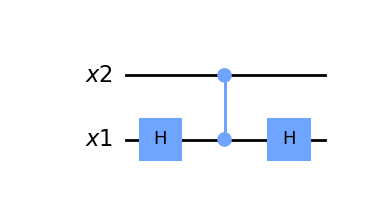
\includegraphics[]{images/Figure_1.png}

\textbf{4.19}

A density matrix of the state $\ket{00},\ket{01},\ket{10},\ket{11}$ will be $\rho = a_1\ket{00}\bra{00} + a_2\ket{01}\bra{01} + a_3\ket{10}\bra{10} +  a_4\ket{11}\bra{11}$ where $a_1^2 + a_2^2 +a_3^2 +a_4^2= 1$. Since the $C-NOT$ gate is
\[U = \begin{bmatrix}
    1 & 0 & 0 & 0 \\
    0& 1 & 0 & 0\\
    0 & 0 & 0 & 1 \\
    0 & 0 & 1 & 0\\
\end{bmatrix}\] and
$U = U^\dag$. We have the evolution of $\rho$ being $ U\rho U  = a_1U\ket{00}\bra{00}U + a_2U\ket{01}\bra{01}U + a_3U\ket{10}\bra{10}U +  a_4U\ket{11}\bra{11}U = a_1\ket{00}\bra{00} + a_2\ket{01}\bra{01} + a_3\ket{11}\bra{11} +  a_4\ket{10}\bra{10}$

\textbf{4.20}

The quantum circuit can be thought of as $(I\otimes H)(H\otimes I)U(I\otimes H)(H\otimes I)$ where $U$ is the $C-NOT$ gate. We then have $(I\otimes H)(H\otimes I)U(I\otimes H)(H\otimes I) = (H\otimes H)U(H\otimes H)$
Since we have \[H\otimes H= \frac{1}{2}\begin{bmatrix}
    1 & 1 & 1 & 1 \\
    1 & -1 & 1 & -1\\
    1 & 1 & -1 & -1 \\
    1 & -1 & -1 & 1\\
\end{bmatrix}\]
We have \[(H\otimes H)U(H\otimes H) =\] \[\frac{1}{4}\begin{bmatrix}
    1 & 1 & 1 & 1 \\
    1 & -1 & 1 & -1\\
    1 & 1 & -1 & -1 \\
    1 & -1 & -1 & 1\\
\end{bmatrix}\begin{bmatrix}
    1 & 0 & 0 & 0 \\
    0& 1 & 0 & 0\\
    0 & 0 & 0 & 1 \\
    0 & 0 & 1 & 0\\
\end{bmatrix}\begin{bmatrix}
    1 & 1 & 1 & 1 \\
    1 & -1 & 1 & -1\\
    1 & 1 & -1 & -1 \\
    1 & -1 & -1 &1\\
\end{bmatrix} = \]
\[\frac{1}{4}\begin{bmatrix}
    1 & 1 & 1 & 1 \\
    1 & -1 & 1 & -1\\
    1 & 1 & -1 & -1 \\
    1 & -1 & -1 & 1\\
\end{bmatrix}\begin{bmatrix}
    1 & 1 & 1 & 1 \\
    1 & -1 & 1 & -1\\
    1 & -1 & -1 & 1 \\
    1 & 1 & -1 & -1\\
\end{bmatrix} =\begin{bmatrix}
    1 & 0 & 0 & 0 \\
    0 & 0 & 0 & 1\\
    0 & 0 & 1 & 0 \\
    0 & 1 & 0 & 0\\
\end{bmatrix}\] 
as required. We are trying to find $U\ket{++}$
Since $(H\otimes H)U(H\otimes H) \ket{00} = (H\otimes H)U\ket{++} $ and $ (H\otimes H)U(H\otimes H) \ket{00} = \ket{00}$, we have $(H\otimes H)U\ket{++} =  \ket{00}$ meaning $(H\otimes H)(H\otimes H)U\ket{++} =  (H\otimes H)\ket{00}$. That in turn means $U\ket{++} = \ket{++}$. The rest follows from similar reasoning.

\textbf{4.21}

We have \[\ket{000}\rightarrow \ket{000}\quad \ket{001} \rightarrow \ket{001}\]\[\ket{010} \rightarrow \ket{010} \quad \ket{011} \rightarrow \ket{011}\] \[\ket{100} \rightarrow \ket{100} \quad \ket{101} \rightarrow\ket{101}\] \[\ket{110} \rightarrow \ket{11}U\ket{0}\quad \ket{111}\rightarrow\ket{11}U\ket{1}\] for the $C^2(U)$ gate. Now consider the right side. We have $\ket{000}$ won't apply any of the controlled gates meaning we are left with $\ket{000}$ after going through the right. For $\ket{001}$ the same can be said because the control parts are in $x_1$ and $x_2$ resulting in $\ket{001}$. For $\ket{010}$, the first $V$ and $V^\dag$ gates are applied resulting in $\ket{01}VV^\dag\ket{0}$. But since $V$ is unitary we have $VV^\dag = I $. This results in $\ket{010}$ still. For $\ket{011}$ we have the same situation as $\ket{010}$ and so we are left with $\ket{011}$. For $\ket{100}$ the first not gate is applied flipping the second qubit to $\ket{1}$ which means $V^\dag$ is applied to the third qubit. Then the second qubit is flipped back to $\ket{0}$. Finally the final $V$ gate to the third qubit. This results in $ \ket{1}XX\ket{0}VV^\dag\ket{0} = \ket{100}$. For $\ket{101}$ we have the same situation as $\ket{100}$ and we are thus left with $ \ket{101}$. For $\ket{110}$, we have $V$ first applied to the third qubit, then $X$ applied to the second, this makes it so that $ V^\dag$ is not applied, X is then applied again to the second qubit and the final $V$ is applied to the third qubit resulting in $ \ket{1}XX\ket{1}VV\ket{0} = \ket{11}U \ket{0}$. For $\ket{111}$ we have the same situation as $\ket{110}$ and thus resulting in $\ket{11}U\ket{1}$. Therefore we can conclude that the two sides are equivalent. 

\textbf{4.22(U)}

Since $V$ is a unitary operator we can express it as  $V = e^{i\alpha}AXBXC$ where $ABC = I$ and are also unitary matrices. That means $ V^\dag =e^{-i\alpha}C^\dag XB^\dag XA^\dag $. We then have

\begin{figure}[H]
    \centering
    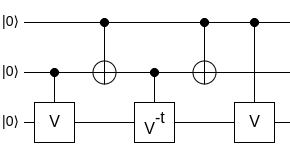
\includegraphics{images/4.22.1.png}
    \label{fig:1}
\end{figure}
is equivalent to 

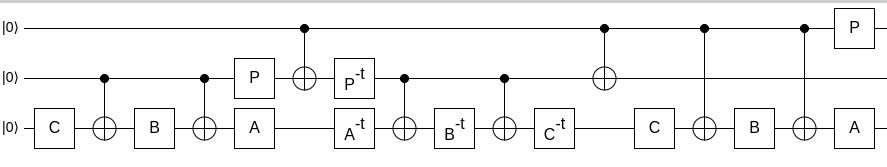
\includegraphics[scale = 0.35]{images/4.22.2.png}

where 
\[P = \begin{bmatrix}
    1 & 0 \\
    0 & e^{i\alpha}
\end{bmatrix}\]
Since $ A$ and $C$ are both unitary, we have $ AA^\dag = I$ and $C^\dag C = I$. This results in 

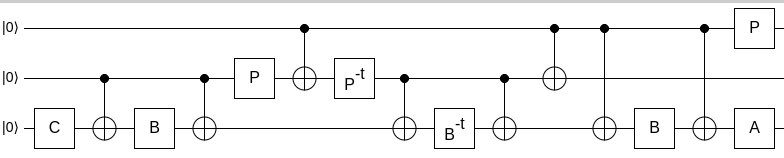
\includegraphics[scale = 0.4]{images/4.22.3.png}

4) this can then be 

\textbf{4.23}

We have 
\[R_{x}(\theta) = \begin{bmatrix}
    \cos(\theta/2) & -i\sin(\theta/2)\\
    -i\sin(\theta/2) & \cos(\theta/2)
\end{bmatrix} =\] \[
e^{i\alpha}R_z(\beta)R_y(\gamma)R_z(\delta) =
\begin{bmatrix}
    e^{i(\alpha- \beta/2 - \delta/2)}\cos(\gamma/2)  & -e^{i(\alpha- \beta/2 + \delta/2)}\sin(\gamma/2) \\
    e^{i(\alpha + \beta/2 - \delta/2)}\sin(\gamma/2) & e^{i(\alpha+ \beta/2 + \delta/2)}\cos(\gamma/2) 
\end{bmatrix} \]
So $\cos(\theta/2) =e^{i(\alpha- \beta/2 - \delta/2)}\cos(\gamma/2)$, $-i\sin(\theta/2) = -e^{i(\alpha- \beta/2 + \delta/2)}\sin(\gamma/2)$, $-i\sin(\theta/2) = e^{i(\alpha + \beta/2 - \delta/2)}\sin(\gamma/2)$, and $\cos(\theta/2) = e^{i(\alpha+ \beta/2 + \delta/2)}\cos(\gamma/2)$. Thus we have \[e^{-i(\alpha+ \beta/2 + \delta/2)}=e^{i(\alpha+ \beta/2 + \delta/2)}\] meaning \[-(\alpha+ \beta/2 + \delta/2) = (\alpha+ \beta/2 + \delta/2)\] which is only true when 
\[(\alpha+ \beta/2 + \delta/2) = 0\]
That would then mean $\gamma = \theta$
and since we have \[-e^{i(\alpha- \beta/2 + \delta/2)} = e^{i(\alpha + \beta/2 - \delta/2)}\] This results in
\[i(\pi + \alpha- \beta/2 + \delta/2)= i(\alpha + \beta/2 - \delta/2)\] and so we have 
\[\pi + \alpha- \beta/2 + \delta/2 =\alpha + \beta/2 - \delta/2 \] resulting in $ \pi = \beta- \delta $.
That then means \[-a - \pi/2 =\delta\quad \beta = \frac{\pi}{2} -\alpha\] Thus we have 
\[R_x(\theta) = e^{i\alpha}R_z\left(\frac{\pi}{2} - \alpha\right)R_y(\theta)R_z\left(-\alpha -\frac{\pi}{2}\right)\]
where $\alpha$ is arbitrary. So we choose $\alpha = 0$ and obtain 
\[R_x(\theta) = R_z\left(\frac{\pi}{2}\right)R_y(\theta)R_z\left(-\frac{\pi}{2}\right)\]We then set \[A = R_z\left(\frac{\pi}{2} \right)R_y\left(\frac{\theta}{2}\right)\quad B = R_y\left(\frac{-\theta}{2}\right)R_z\left(0\right)\quad C = R_z\left(\frac{-\pi}{2}\right)\]
and obtain the decomposition \[R_x(\theta) = e^{\alpha}AXBXC =R_z\left(\frac{\pi}{2} \right)R_y\left(\frac{\theta}{2}\right)XR_y\left(-\frac{\theta}{2}\right)XR_z\left(-\frac{\pi}{2}\right)\] There does not seem to be any way to make this have only two single qubit gates. Now consider $R_y(\theta)$, we have $ R_y(\theta) = e^{i\alpha}R_z(\beta)R_y(\gamma)R_z(\delta)$, where clearly, $\alpha = 0$, $\beta = 0$, $\gamma = \theta$, and $\delta = 0$. By letting $ A = R_z(0)R_y(\theta/2) $, $B = R_y(-\theta/2)R_z(0)$, and $C = R_z(0)$. Thus we have 
\[R_y(\theta) = e^{i\alpha}AXBXC = R_y(\theta/2) X R_y(-\theta/2) X\] which only has two single qubit gates.

\textbf{4.25}

1)

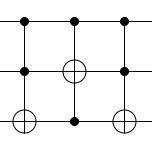
\includegraphics[scale=0.5]{images/4.25.png}

represents a fredkin gate, as can be seen by supplying all possible inputs. 

2) 

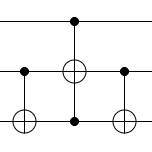
\includegraphics[scale = 0.5]{images/4.25.1.png}

represents a fredkin gate as well. For the input $0,0,0$, we have $0,0,0$ after the first cnot, then after the toffoli gate, we still have $0,0,0$ and finally after the second cnot, we are left with $0,0,0$ as required. For $0,0, 1$, we have after the first cnot, $0,0,1$, after the toffoli, $0,0,1$, and after the second cnot $0,0,1$ as required. For $0,1,0$ we have after the first cnot, $ 0,1,1$, after the toffoli, $0,1,1$, and after the second cnot $0,1,0$ as required. For $0,1,1$, we have $0,1,0$ after the first cnot, then $0,1,0$ after the toffoli, and after the second cnot $0,1,1$ as required. For $1,0,0$ we have $1,0,0$ after the first cnot, $1,0,0$ after the toffoli, and $ 1,0,0$ after the second cnot as required. For $1,0,1$, we have after the first cnot, $1,0,1$ after the toffoli, $ 1,1,1$ and after the second cnot, $1,1,0$ as required. For $ 1,1,0$, we have after the first cnot, $ 1,1,1$, after the toffoli, we have $ 1,0,1$ and after the second cnot, $1,0,1$ as required. For $1,1,1$ we have after the first cnot, $1,1,0$, after the toffoli $1,1,0$ and after the second cnot $ 1,1,1$ as required. Thus we can conclude that the above circuits action is the same as a fredkin gate.

3)

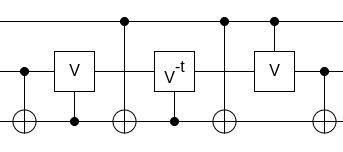
\includegraphics[scale = 0.5]{images/4.25.2.png}

where $V  = (1-i)(I+iX)/2$ also represents a fredkin gate this can be simplified to 

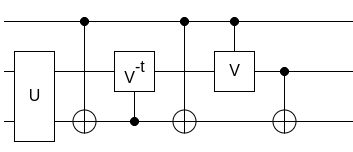
\includegraphics[scale = 0.5]{images/4.25.3.png} 

Where $U$ represents the application of the $cnot$ and $cv$ gates.

4) 

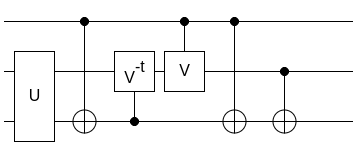
\includegraphics[scale = 0.5]{images/4.25.4.png}

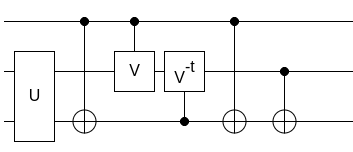
\includegraphics[scale = 0.5]{images/4.25.5.png}

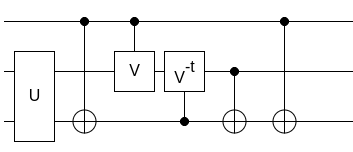
\includegraphics[scale = 0.5]{images/4.25.6.png}

The above are equivalent to a fredkin gate. The first one because the cnot and cv gates don't affect each other, allowing it to be swapped. The second because of the unitary nature of V, thus making it normal and commutes with each other. The third is because the control qubits are not affected and $X$ commutes with itself. From the above we can replace the $cv^{-t}$ and cnot gate with a single two qubit gate $M$ and obtain

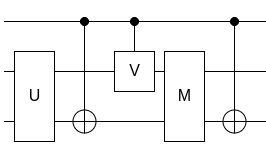
\includegraphics[scale = 0.5]{images/4.25.7.png}

which has only five 2 qubit gates as required.

\textbf{4.27}

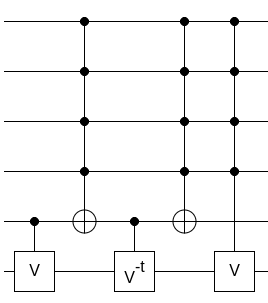
\includegraphics[scale = 0.5]{images/4.27.png}

Is equivalent since this is basically the same as the ccu gate except conditional on 5 qubits rather than 2.

\textbf{4.32}

We would have after measurement, but with no knowledge of the measurement, the state $ \rho' =  \sum_m p(m)\rho_m = \sum_m M_m \rho M_m^\dag = P_0\rho P_0 + P_1 \rho P_1$. Since we have by schmidt decomposition \[\rho = \sum_{i} \lambda_i^2\ket{i_ai_b}\bra{i_ai_b} =\sum_{i} \lambda_i^2\ket{i_a}\bra{i_a}\otimes \ket{i_b}\bra{i_b}\] then \[tr_2(\rho) = \sum_i\lambda_i^2\ket{i_a}\bra{i_a}\braket{i_b|i_b} = \sum_i\lambda_i^2\ket{i_a}\bra{i_a}\]since $\ket{i_b}$ is orthonormal. Also \[tr_2(\rho') = tr_2(P_0\rho P_0 + P_1\rho P_1) =\] \[tr_2\left(\sum_{i} \lambda_i^2\ket{i_a}\bra{i_a}\otimes P_0\ket{i_b}\bra{i_b}P_0 + \sum_{i} \lambda_i^2\ket{i_a}\bra{i_a}\otimes P_1\ket{i_b}\bra{i_b}P_1\right) = \]
\[\sum_i\lambda_i^2\ket{i_a}\bra{i_a}(tr(P_0\ket{i_b}\bra{i_b}P_0) + tr(P_1\ket{i_b}\bra{i_b}P_1)) =  \]
\[\sum_i\lambda_i^2\ket{i_a}\bra{i_a}(tr(\ket{0}\bra{0}\ket{i_b}\bra{i_b}\ket{0}\bra{0}) + tr(\ket{1}\bra{1}\ket{i_b}\bra{i_b}\ket{1}\bra{1})) = \]
\[\sum_i\lambda_i^2\ket{i_a}\bra{i_a}(\bra{0}\ket{i_b}\bra{i_b}\ket{0} + \bra{1}\ket{i_b}\bra{i_b}\ket{1})\] But we have $i_b = a\ket{0} + b\ket{1}$ and $\braket{i_b | i_b} = 1$. Thus $a\overline{a} + b\overline{b} = 1$. Then $\bra{0}\ket{i_b}\bra{i_b}\ket{0} + \bra{1}\ket{i_b}\bra{i_b}\ket{1} = \overline{a}a + \overline{b}b  = 1$ meaning 
\[tr_2(\rho') = \sum_i\lambda_i^2\ket{i_a}\bra{i_a}\] and thus we can conclude $tr_2(\rho') = tr_2(\rho)$ as required.

\textbf{4.33}

We have from the circuit \[\ket{00} \rightarrow \frac{1}{\sqrt{2}}(\ket{00} + \ket{10})\quad \ket{01} \rightarrow \frac{1}{\sqrt{2}}(\ket{01} + \ket{11})\]
\[\ket{10} \rightarrow \frac{1}{\sqrt{2}}(\ket{01} - \ket{11}) \quad \ket{11} \rightarrow \frac{1}{\sqrt{2}}(\ket{00} - \ket{10})\]
Now by inputting the bell states we then have 
\[\frac{1}{\sqrt{2}}(\ket{00}+\ket{11}) \rightarrow \frac{1}{2}(\ket{00} + \ket{10} + \ket{00} - \ket{10}) = \ket{00}\]
\[\frac{1}{\sqrt{2}}(\ket{01} + \ket{10}) \rightarrow \frac{1}{2}(\ket{01} + \ket{11} + \ket{01} - \ket{11}) = \ket{01}\]
\[\frac{1}{\sqrt{2}} (\ket{00} - \ket{11})\rightarrow \frac{1}{2}(\ket{00}+\ket{10} -\ket{00})+ \ket{10}) = \ket{10}\]
\[\frac{1}{\sqrt{2}}(\ket{01} - \ket{10}) = \frac{1}{2}(\ket{01} + \ket{11} - \ket{01} + \ket{11}) = \ket{11}\] Thus measurement of the computational basis is equivalent to measuring in the bell basis.

Because we have after a measurement, the state \[\frac{M_m\ket{\psi}}{\sqrt{\bra{\psi}M_m^\dag M_m \ket{\psi}}}\] So what we want is, when inputting the bell states, the measurements should take it to the same bell space This is true when $M_{00} = \ket{\beta_{00}}\bra{\beta_{00}}$, $M_{01} = \ket{\beta_{01}}\bra{\beta_{01}}$, $M_{10} = \ket{\beta_{10}}\bra{\beta_{10}}$, and $M_{11} = \ket{\beta_{11}}\bra{\beta_{1}}$ where $\beta$ are the bell states. Since these are all projective measurements, we have their $POVM$ being the same since $M_mM_m^\dag = E_m$.

\textbf{4.34}

We have after each gate

\[\ket{0\psi_{in}}\rightarrow \frac{1}{\sqrt{2}}(\ket{0\psi_{in}} + \ket{1\psi_{in}})\rightarrow \frac{1}{\sqrt{2}}(\ket{0\psi_{in}} + \ket{1(U\psi_{in})})\rightarrow \]
\[\frac{1}{\sqrt{2}}(\ket{(H0)\psi_{in}} + \ket{(H1)(U\psi_{in})}) =\frac{1}{2}(\ket{0\psi_{in}} +\ket{1\psi_{in}}  + \ket{0(U\psi_{in})}- \ket{1(U\psi_{in})})\] Thus we would have when measuring $\ket{0}$
\[\ket{\psi_{out}} = (I+U)\ket{\psi_{in}}\] and when measuring $\ket{1} $
\[\ket{\psi_{out}} = (I-U)\ket{\psi_{in}}\] We also have for $\ket{0}$ $U\ket{\psi_{out}} = U(I + U)\ket{\psi_{in}} = (U+ U^2)\ket{\psi_{in}} =(U+I)\ket{\psi_{in}} = \ket{\psi_{out}} $ or $ U\ket{\psi_{out}} U(I-U)\ket{\psi_{in}} =(U-U^2)\ket{\psi_{in}} =(U-I)\ket{\psi_{in}} = -\ket{\psi_{out}}$. Meaning $\ket{\psi_{out}}$ are eigenvectors in both cases and $\ket{0}$ corresponds with the eigenvalue $1$, while $\ket{1}$ with the eigenvalue $-1$.

\textbf{4.35}

We have in the first circuit

\[\ket{00}\rightarrow \ket{(P_00/\sqrt{\bra{0}P_0\ket{0}})0} = \ket{00}\]
\[\ket{01} \rightarrow \ket{(P_00/\sqrt{\bra{0}P_0\ket{0}})0} = \ket{01}\]
\[\ket{10} \rightarrow \ket{1(U0)}\rightarrow \ket{(P_11/\sqrt{\bra{1}P_1\ket{1}})(U0)} = \ket{1(U0)}\]
\[\ket{11} \rightarrow \ket{1(U1)}\rightarrow \ket{(P_11/\sqrt{\bra{1}P_1\ket{1}})(U1)} = \ket{1(U1)}\]

From the second circuit we have 
\[\ket{00}\rightarrow \ket{(P_00/\sqrt{\bra{0}P_0\ket{0}})0} = \ket{00}\]
\[\ket{01} \rightarrow \ket{(P_00/\sqrt{\bra{0}P_0\ket{0}})0} = \ket{01}\]
\[\ket{10} \rightarrow \ket{(P_11/\sqrt{\bra{1}P_1\ket{1}})0} = \ket{10}\rightarrow\ket{1(U0)} \]
\[\ket{11}\rightarrow \ket{(P_11/\sqrt{\bra{1}P_1\ket{1}})1} = \ket{11} \rightarrow \ket{1(U1)}\]
and thus we can conclude that the two circuits are equivalent as required

\textbf{4.36}

consider the circuit

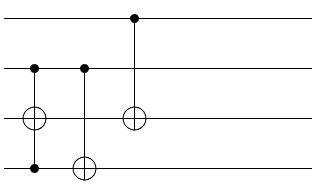
\includegraphics[scale = 0.5]{images/4.36.png}

where the top two qubits represents $x$ and the bottom two represents $y$. This circuit results in $\ket{x,y}\rightarrow \ket{x,x+y \ mod \ 4}$

\textbf{4.40}

We have \[E(R_{\hat{n}}(\alpha),R_{\hat{n}}(\alpha+\beta)) = \max_{\ket{\psi}}|(R_{\hat{n}}(\alpha) - R_{\hat{n}}(\alpha+\beta))\ket{\psi}|\] 
The maximum difference occurs when we have a state that is perpendicular to the axis of rotation. 

\textbf{4.41}

We have 
\[\ket{00\psi}\xrightarrow{H,H} \frac{1}{\sqrt{2}}(\ket{0(H0)\psi} + \ket{1(H0)\psi}) =\frac{1}{2}(\ket{00\psi} +\ket{01\psi}  + \ket{10\psi}+\ket{11\psi})\xrightarrow{ccnot} \]
\[\frac{1}{2}(\ket{00\psi} +\ket{01\psi}  + \ket{10\psi}+\ket{11(X\psi)})\xrightarrow{S}\]
\[\frac{1}{2}(\ket{00(S\psi)} +\ket{01(S\psi)}  + \ket{10(S\psi)}+\ket{11(SX\psi)})\xrightarrow{ccnot}\]
\[\frac{1}{2}(\ket{00(S\psi)} +\ket{01(S\psi)}  + \ket{10(S\psi)}+\ket{11(XSX\psi)})\xrightarrow{H,H}\]
\[\frac{1}{2\sqrt{2}}(\ket{0(H0)(S\psi)}+\ket{1(H0)(S\psi)} +\ket{0(H1)(S\psi)} + \ket{1(H1)(S\psi)}  +\]\[\ket{0(H0)(S\psi)} -\ket{1(H0)(S\psi)}+\ket{0(H1)(XSX\psi)}-\ket{1(H1)(XSX\psi)}) = \]
\[\frac{1}{2\sqrt{2}}(2\ket{0(H0)(S\psi)} +\ket{0(H1)(S\psi)} + \ket{1(H1)(S\psi)} +\]\[\ket{0(H1)(XSX\psi)}-\ket{1(H1)(XSX\psi)}) = \]
\[\frac{1}{4}(2\ket{00(S\psi)} + 2\ket{01(S\psi)}+\ket{00(S\psi)}-\ket{01(S\psi)} + \ket{10(S\psi)}-\ket{11(S\psi)} +\]\[\ket{00(XSX\psi)} -\ket{01(XSX\psi)}-\ket{10(XSX\psi)} + \ket{11(XSX\psi)}) = \]
\[\frac{1}{4}(3\ket{00(S\psi)} + \ket{01(S\psi)} + \ket{10(S\psi)}-\ket{11(S\psi)} +\]\[\ket{00(XSX\psi)} -\ket{01(XSX\psi)}-\ket{10(XSX\psi)} + \ket{11(XSX\psi)}) = \]
\[\frac{1}{4}(\ket{00((3S + XSX)\psi)} + \ket{01((S-XSX)\psi)} +\]\[\ket{10((S-XSX)\psi)} + \ket{11((XSX-S)\psi)})\] Thus when both measurement outcomes are $0$, we have $\frac{1}{4}(3S + XSX)$ being applied to the final qubit.
But \[\frac{1}{4}(3S + XSX) = \frac{1}{4}\left(3\begin{bmatrix}
    1 & 0 \\
    0 & i
\end{bmatrix} + \begin{bmatrix}
    0 & 1\\
    1 & 0\\
\end{bmatrix}\begin{bmatrix}
    1 & 0\\
    0 & i\\
\end{bmatrix}\begin{bmatrix}
    0 & 1\\
    1 & 0\\
\end{bmatrix}\right) = \]
\[\frac{1}{4}\left(3\begin{bmatrix}
    1 & 0 \\
    0 & i
\end{bmatrix} + \begin{bmatrix}
    i & 0 \\
    0 & 1
\end{bmatrix}  \right) = \frac{1}{4}\begin{bmatrix}
    3+i & 0 \\
    0 & 1+3i
\end{bmatrix} = \]\[\frac{\sqrt{10}}{4}\begin{bmatrix}
    \frac{3}{\sqrt{10}}+i\frac{1}{\sqrt{10}} & 0 \\
    0 & \frac{1}{\sqrt{10}}+i\frac{3}{\sqrt{10}}
\end{bmatrix} \]
So by setting $Ae^{i\theta/2} = \frac{3}{\sqrt{10}}+i\frac{1}{\sqrt{10}}$ and $ Ae^{-i\theta/2} =\frac{1}{\sqrt{10}}+i\frac{3}{\sqrt{10}} $. Then \[A^2 = \left(\frac{3}{\sqrt{10}}+i\frac{1}{\sqrt{10}}\right)\left(\frac{1}{\sqrt{10}}+i\frac{3}{\sqrt{10}}\right) = \frac{3}{10} + i - \frac{3}{10} = i= \left(\frac{1}{\sqrt{2}} +\frac{i}{\sqrt{2}}\right)^2\]
Therefore 
\[A = \frac{1}{\sqrt{2}}+\frac{i}{\sqrt{2}} = e^{i\pi/4}\]
making $ e^{i\theta/2} =e^{-i\pi/4}(\frac{3}{\sqrt{10}}+i\frac{1}{\sqrt{10}}) $ and $ e^{-i\theta/2} = e^{-i\pi/4}(\frac{1}{\sqrt{10}}+i\frac{3}{\sqrt{10}})$. Thus we have
\[\frac{1}{4}(3S + XSX) = \frac{\sqrt{10}e^{i\pi/4}}{4}\begin{bmatrix}
    e^{-i\pi/4}\left(\frac{3}{\sqrt{10}}+i\frac{1}{\sqrt{10}}\right) & 0 \\
    0 & e^{-i\pi/4}\left(\frac{1}{\sqrt{10}}+i\frac{3}{\sqrt{10}}\right)
\end{bmatrix}\]
which is indeed $R_z(\theta)$ with a global phase shift.
We also have \[e^{i\theta} =\frac{\frac{3}{\sqrt{10}}+i\frac{1}{\sqrt{10}}}{\frac{1}{\sqrt{10}}+i\frac{3}{\sqrt{10}}} = \frac{\frac{3}{\sqrt{10}}+i\frac{1}{\sqrt{10}}}{\frac{1}{\sqrt{10}}+i\frac{3}{\sqrt{10}}} \left(\frac{\frac{1}{\sqrt{10}}-i\frac{3}{\sqrt{10}}}{\frac{1}{\sqrt{10}}-i\frac{3}{\sqrt{10}}}\right) = \frac{3}{10} + \frac{i}{10} -\frac{9i}{10} + \frac{3}{10} = \frac{3}{5}+\frac{4}{5}i \]
Thus $\cos(\theta) = 3/5$ as required. In the other cases we have $\pm(S-XSX)$ applied to the final qubit. Since
\[S-XSX = \begin{bmatrix}
    1 & 0 \\
    0 & i
\end{bmatrix} - \begin{bmatrix}
    i & 0 \\
    0 & 1
\end{bmatrix} = -iZ\]
we have an application of $Z$ with global phase shift. The probability of both measurements being $0$ is \[\frac{1}{16}\braket{00(\sqrt{10}e^{i\pi/4}R_z(\theta)\psi)|00(\sqrt{10}e^{i\pi/4}R_z(\theta)\psi)} =\]\[ \frac{10}{16}\braket{00(R_z(\theta)\psi)|00(R_z(\theta)\psi)} = \frac{5}{8}\]
as required

If the resulting measurements is not $00$, we can apply a $Z$ gate to the final qubit in order to get the final qubit back to its initial state. Then we can apply the circuit again in order to try and obtain $00$. More and more applications of this procedure will result in higher probability of achieving $R_z(\theta)$ since the probability of $R_z(\theta)$ is $1-(\frac{3}{8})^n$, where $n$ is the number of times the circuit is applied. Thus as $n\rightarrow \infty$, the probability of the desired gate goes to $1$.





